%%%%%%%%%%%%%%%%%%%%%%%%%%%%%%%%%%%%%%%%%%%%%%%%%%%%%%%%%%%%%%%%%%%%%%%%%%%%%%%%%%%%
% Do not alter this block (unless you're familiar with LaTeX
\documentclass{article}
\usepackage[margin=1in]{geometry} 
\usepackage{amsmath,amsthm,amssymb,amsfonts, fancyhdr, color, comment, graphicx, environ}
\usepackage{xcolor}
\usepackage{mdframed}
\usepackage[shortlabels]{enumitem}
\usepackage{indentfirst}
\usepackage{hyperref}
\usepackage{algorithm}% http://ctan.org/pkg/algorithm
\usepackage[noend]{algpseudocode}% http://ctan.org/pkg/algorithmicx
\usepackage{graphicx}
\hypersetup{
    colorlinks=true,
    linkcolor=blue,
    filecolor=magenta,      
    urlcolor=blue,
}


\pagestyle{fancy}


\newenvironment{problem}[2][Problem]
    { \begin{mdframed}[backgroundcolor=gray!20] \textbf{#1 #2} \\}
    {  \end{mdframed}}

% Define solution environment
\newenvironment{solution}
    {\textit{Soln:}}
    {}

\renewcommand{\qed}{\quad\qedsymbol}

% prevent line break in inline mode
\binoppenalty=\maxdimen
\relpenalty=\maxdimen

\graphicspath{ {./images/} }

%%%%%%%%%%%%%%%%%%%%%%%%%%%%%%%%%%%%%%%%%%%%%
%Fill in the appropriate information below
\lhead{Anmol Lingan Gouda Patil}
\rhead{COT5405} 
\chead{\textbf{Homework 1  Due: 11 Oct 2021 11:59pm}}
%%%%%%%%%%%%%%%%%%%%%%%%%%%%%%%%%%%%%%%%%%%%%
% \RestyleAlgo{ruled}
\begin{document}

\begin{mdframed}[backgroundcolor=yellow!20]
\textbf{Design and implement an algorithm to find a cycle (just one cycle) in an undirected graph.} 
\end{mdframed}

\begin{problem}{1}
\textbf{[10 pts]} Design a correct algorithm and show it in pseudo-code 
\end{problem}
\begin{solution}
\begin{algorithm}
\caption{Detect Cycle Depth First Search}\label{dfs}
\begin{algorithmic}[1]
% \KwResult{A boolean as to whether a cycle exists or not}
\Procedure{IsCyclic}{$G$}
% initialization\;
    \For{\texttt{each vertex $v$ in $G$}}
        \State \texttt{$visited[u] \gets false$}
    \EndFor
    
    \For{\texttt{each vertex $v$ in $G$}}
        \If {$v$ is not visited}
            \If {$DFSUtil(G, v, -1, visited) = true$}
                \State \Return \texttt{$true$}
            \EndIf
        \EndIf
    \EndFor
    \State \Return $false$
\EndProcedure
\newline
\Procedure{DFSUtil}{$G,v,parent,visited$}
    \State \texttt{$visited[v] \gets true$}
    \For{\texttt{each neighboring vertex $u$ of $v$}}
        \If{$u$ is not visited}
            \If {$DFSUtil(G, u, v, visited) = true$}
                \State \Return \texttt{$true$}
            \EndIf
        \Else
            \If {$u \ne parent$} \Comment{A backedge}
                \State \Return $true$
            \EndIf
        \EndIf
    \EndFor
    \State \Return $false$
\EndProcedure
\end{algorithmic}
\end{algorithm}

\end{solution}

\begin{problem}{2}
\textbf{[10 pts]} Provide proof of the algorithm's correctness. 
\end{problem}
\begin{solution}
To prove the correctness of the algorithm above that uses DepthFirstSearch, let us first prove the following:
\newline \textbf{\textit{Lemma1:}} A directed graph contains a cycle if and only if DepthFirstSearch on that graph classifies some edges as back edges.
\begin{proof}
Suppose G has a back edge (v,u).
Then v is a descendant of u in the DFS forest.
Therefore, a cycle from u to v in G can be obtained by going from u to v via tree edges and then going from v to u via (v,u).
Suppose G has a cycle C.
Let u be the first vertex in C to be discovered.
Since there is a path from u to all other vertices in C and those vertices are white when u is discovered, all those vertices will become descendants of u by the white path theorem.
Since u is in a cycle C, there is at least one vertex v in C such that (v,u) is in G.
Since v is a descendant of u, (v,u) will be classified as a back edge. Therefore, if G is cyclic, it has a back edge.\end{proof}
\begin{center}
The algorithm $Detect Cycle Depth First Search$ returns true as soon as it encounters a back edge. As we know that using $Lemma 1$ a graph has a cycle if it has a back edge then the algorithm always finds a cycle if there is one.
\end{center}
\end{solution}

\begin{problem}{3}
\textbf{[10 pts]} Find and prove the algorithm's running time.
\end{problem}
\begin{solution}
The time complexity of the algorithm above is O(V) where V is the number of nodes.
\begin{itemize}
\item A tree contains V-1 edges and a cycle should contain atleast V edges. \item The above algorithm visits every node once.
\item If there is a cycle, the above algorithm visits atmost V nodes before discovering a back edge and terminates, hence V operations.
\item If there is no cycle it traverses all nodes only once before terminating, also V operations.
\item With running time linearly dependent on the size of vertices or the number of operations, the time complexity hence would be O(V)
\end{itemize}
\end{solution}

\begin{problem}{4}
\textbf{[20 pts]} Implement the algorithm in a compiled language
\begin{enumerate}
    \item Write a graph generator.
    \item Write test code to validate that the algorithm finds cycles.
    \item Test the algorithm for increasing graph sizes.
    \item Plot the running time as a function of size to verify that the asymptotic complexity in step 3 matches experiments.
\end{enumerate}
\end{problem}
\begin{solution}
Running time as a function of size to verify the asymptotic complexity.
\begin{figure}[h]
    \centering
    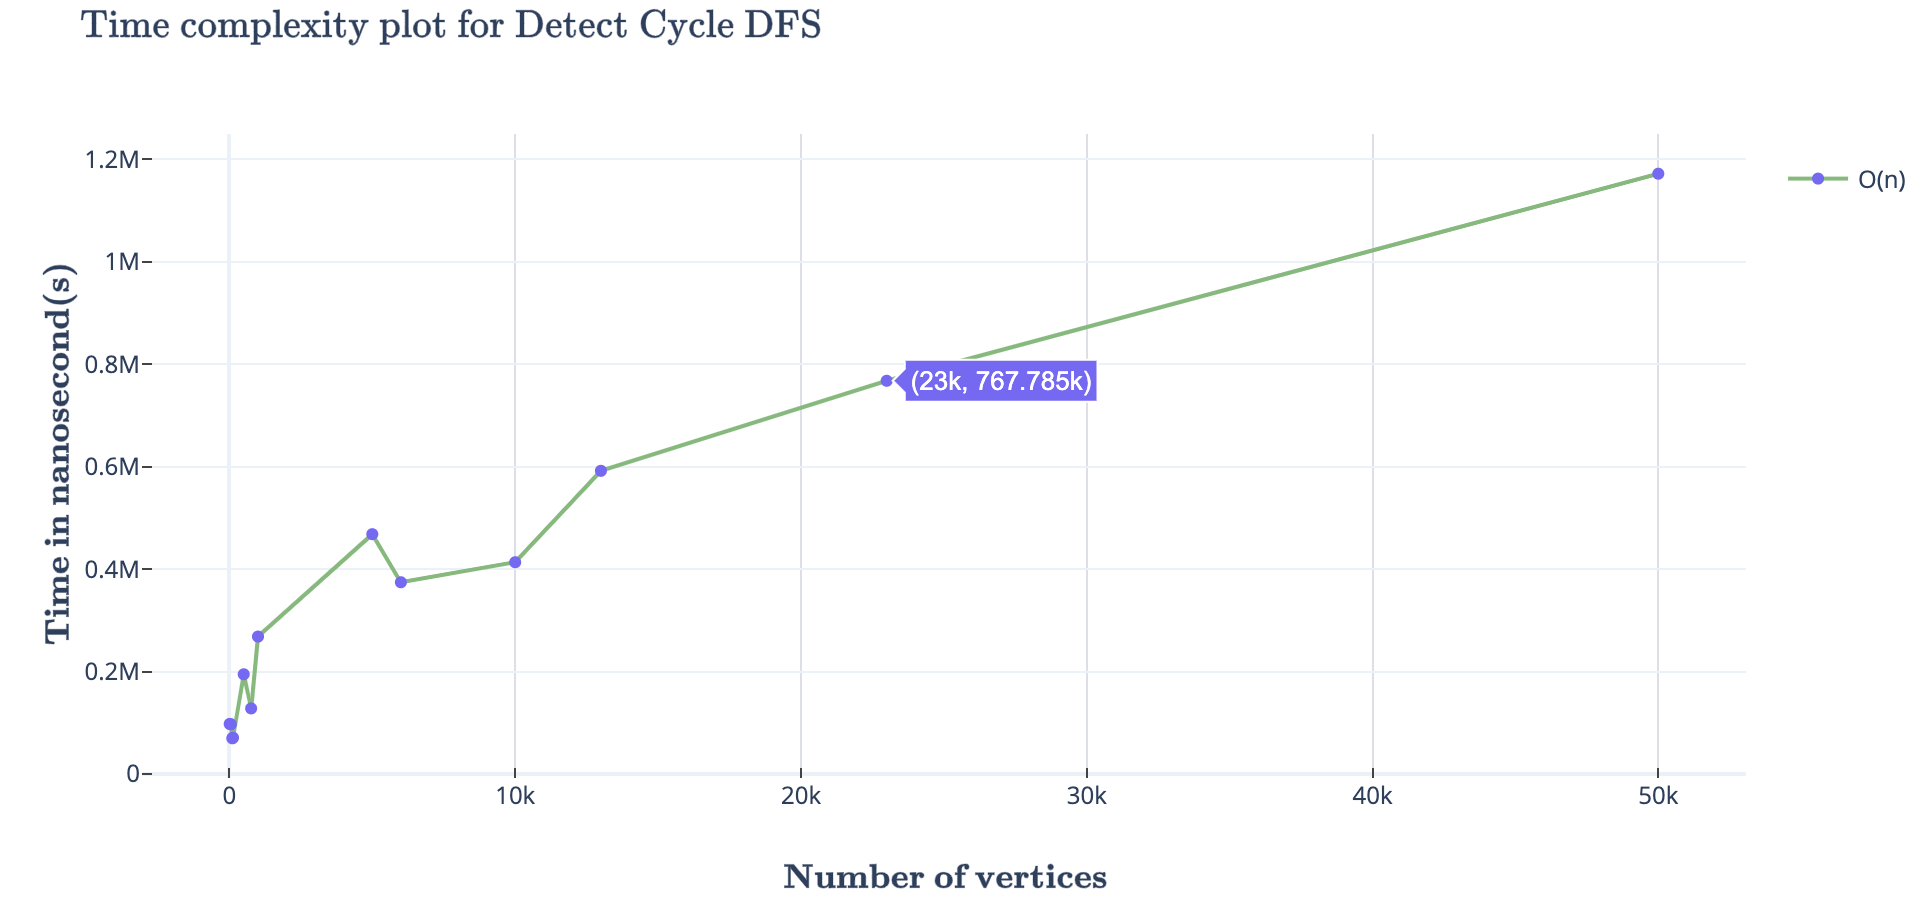
\includegraphics[scale=0.5]{Alg-1}
    \caption{Detect Cycle Depth First Search performance}
    \label{fig:my_label}
\end{figure}
\end{solution}
\end{document}
